\chapter{绪论}

\section{福斯特共振能量转移(FRET)}

\subsection{FRET原理概述}
1948年,Förster首次阐述了福斯特共振能量转移(Förster Resonance Energy Transfer,FRET)理论\upcite{forster1948zwischenmolekulare}。
FRET是指处于激发态的供体分子(Donor)通过偶极子间相互作用将一部分能量以非辐射的形式转移给邻近处于基态的受体(Acceptor)分子(供受体之间的距离$R$在0至10 nm)\upcite{lakowicz2006principles}。
FRET 的发生会使得供体的荧光淬灭和受体的荧光增强,其中由于发生FRET而增强受体荧光称为敏化发射荧光。
FRET技术突破传统观测局限,精准解析分子间相互作用与距离\upcite{yung1973relationship}。
在细胞生物学微观环境里,FRET技术可被用作一种“分子尺”,可以检测纳米尺度上的生物分子动态,从而进一步研究其结构与功能。
因而,FRET技术在细胞生物学多领域,如细胞信号转导、蛋白质相互作用探测等广泛应用。
\begin{figure}[htbp]
    \centering
    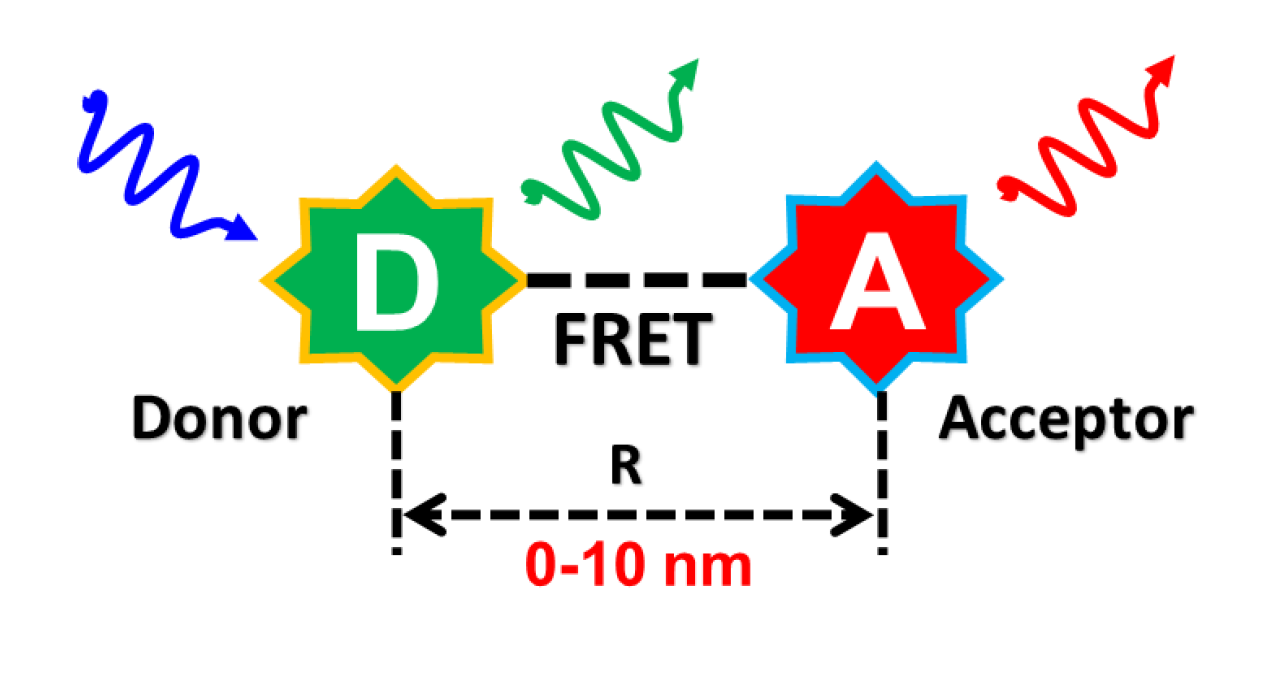
\includegraphics[width=0.5\linewidth]{../figures/1/1_FRET过程示意图.png}
    \caption{FRET过程示意图}
    \label{fig:fret}
\end{figure}

理论和实验证明,当供受体荧光分子的距离为$r$时,它们之间的能量转移速率由下式给出\upcite{yekta1995dipole}:
\begin{equation}
    k_T(r)=\frac{1}{\tau_D}(\frac{R_0}{r})^6, \label{eq:1-1}
\end{equation}
其中$\tau_D$是供体荧光寿命,$R_0$为Förster半径,由下式表示:
\begin{equation}
    R_0^6=8.79\times{10^{-5}}(n^{-4}Q_DJ(\lambda)\kappa^2)(\text{in~} \mbox{\AA}^6),
\end{equation}
上式中,$n$表示介质的折射率,$Q_D$表示供体的量子产率,$J(\lambda)$是光谱重叠积分,$\kappa^2$是方向因子,表示供、受体偶极子的相对方向,一般在自由状态下取$\kappa^2=2/3$。FRET发生需要满足三个条件:(1)$r$的数值在$R_0$附近,约0-10nm;(2)供体的发射谱与受体的吸收谱有超过30\%的重叠;(3)供、受体偶极子方向不互相垂直。

FRET效率($E$)定义为供体转移给受体的能量与供体发射的总能量的比例,是用来衡量FRET程度的指标,其主要和分子间距和荧光团光谱的重叠度有关。光谱有部分重叠的供受体分子间距越小,能量转移就越高效。其计算式为:
\begin{equation}
    {E}=\frac{k_T(r)}{k_T(r)+\tau^{-1}_{D}},
\end{equation}
将公式\ref{eq:1-1}代入,可以看出$E$与$r$的六次方成反比的关系:
\begin{equation}
    E=\frac{R_0^6}{R_0^6+r^6}=\frac{1}{1+(r/R_0)^6}.
\end{equation}

\subsection{FRET在生物学中的应用}

FRET发生的条件是供、受体分子之间的距离$r$在0 - 10nm之间,这使得FRET技术成为一种“纳米尺”,能够有效地测量纳米级的分子间距。
FRET技术在研究生物蛋白相互作用、大分子构象变化、信号通路中的蛋白质调节机制等方面得到了广泛的应用\upcite{2020Single, wu2018translocation, shrestha2015understanding}。

FRET技术应用到各种生物研究中的重要前提是荧光蛋白的发展\upcite{chudakov2010fluorescent}。
1962 年,第一种绿色荧光蛋白(Green Fluorescent Protein, GFP)在维多利亚水母中被发现,由于荧光蛋白的无毒性以及稳定遗传性,可以利用基因转导技术将荧光蛋白接到感兴趣的蛋白质分子上,借助显微成像技术实时观察活细胞中目标蛋白的转位以及信号传递等生物问题\upcite{shimomura2009discovery}。
随着基因技术的发展,最先发现的GFP 蛋白被改造出了多种GFP突变体,多种荧光蛋白的出现为同时追踪多个蛋白质分子间的相互作用和多种蛋白质的共定位等复杂的生物问题提供了必要条件,使得基于FRET显微成像技术在分子生物学和以及生物物理学的活细胞在体研究得到了广泛的应用\upcite{sekar2003fluorescence}。

FRET定量分析方法的发展,如$3^3$-FRET(Three-cube FRET)、E-FRET(Emission FRET)和FRET双杂交分析(FRET Two-hybrid Assay)等,帮助研究人员从独特的角度研究细胞内蛋白质等大分子的相互作用\upcite{erickson2001preassociation,zal2004photobleaching}。
2016年,Ben-Johny等人利用FRET双杂交分析技术定量研究了钙离子通道与钙调蛋白之间的结合,发现当细胞内钙离子浓度较低时,一个钙调蛋白与一个钙离子通道结合;当细胞内钙离子浓度较高时,一个钙离子通道可以同时结合两个钙调蛋白\upcite{ben-johny2016}。
杨方方等人利用FRET双杂交实验,研究了Bcl-2家族的四种抗凋亡或促凋亡蛋白(即Bcl-xL、Bad、Bax和tBid)在健康细胞和凋亡细胞中的相互作用。\upcite{yang2020stoichiometry}。
李小梅等人使用双杂交FRET成像等技术对L型钙通道C末端编码肽进行了定量研究,证明了Calmudolin的多种变体均通过与钙调素竞争,抑制钙通道的基本功能\upcite{yang2022cytosolic}。

基于FRET技术在活细胞内实时监测钙离子的动态变化操作简单,灵敏度更高。
Cornea 等在2009利用荧光共振能量转移技术研究了钙调蛋白(CaM)与骨骼肌 Ryanodine 受体(RyR1)的结合模式\upcite{cornea2009fret}。
2020年Yoon等开发了一种基于 EGFP 和 Fusion Red 的新型 FRET 钙传感器(FRET-GF-PRed),并结合高频超声(HFU)技术实现了单细胞水平的精准刺激与成像\upcite{yoon2020fret}。
Yi等人开发红色电压指示剂 Cepheid1,利用 eFRET 技术实现单细胞电活动与钙信号同步监测,揭示了胰腺细胞电振荡与钙波动的时空关联\upcite{han2023bright}。

FRET还可用于检测酶的活性\upcite{carmona2009use, walter2021coumarin}。
酶支配着生物体内的新陈代谢、营养和能量转换等许多催化过程,影响着生物体内许多信号转导过程。
Cheppali等利用单分子三色 FRET 监测 NSF 酶解聚 SNARE 复合体的过程,揭示其解聚存在两条路径,澄清了酶作用的中间状态机制\upcite{cheppali2025single}。
樊林玮等通过 FRET 传感器发现机械牵张激活 cPLA2,抑制脂肪酸氧化酶活性,通过调控转录因子 YY1 影响血管平滑肌细胞功能\upcite{fan2025mechanical}。

在疾病诊断方面,FRET 技术在药物疗效评估等方面同样具有重要意义\upcite{song2011development, sun2021recent,双杂交药筛}。
2014年,Bozza等人通过设计特定的 FRET 生物传感器,能够直接反映癌症药物诱导癌细胞凋亡的效果,为药物的研发和筛选提供了有力的工具,避免了因无法区分细胞死亡和生长抑制而导致的结果偏差\upcite{bozza2014use}。

\subsection{基于受体敏化发射的FRET定量测量方法(E-FRET)}

受限于实验仪器和样本的准备,早期的FRET测量方式都只能基于定性或半定量测量\upcite{awais2004A,Aye2009Fluorescent}。
复杂实验条件的校正,需要使用表达特定荧光蛋白的细胞进行校正,而蛋白质在细胞中的表达又受到表达的成熟度、胞内的微环境等多种因素制约\upcite{liu2018influence}。

基于受体敏化发射的通道方法(E-FRET)具有测量速度快、无损伤的特性,被公认是最适合用于活细胞动态监测的FRET半定量检测技术\upcite{erickson2001preassociation}。
E-FRET方法需要对实验系统响应和荧光团的光学性质进行严格的校准,一般通过提前测量多个参照样本,然后保持在整个实验过程中系统的稳定和实验条件的一致。
E-FRET方法需要3个Cube组成的3个通道,分别实现供体激发供体收集(DD通道)、供体激发受体收集(DA通道)和受体激发受体收集(AA通道)。
受体的敏化荧光从DA通道测得($I_{DA}$图像),但实际上$I_{DA}$图像包含有供体转移到受体的敏化荧光、供体激发光直接激发受体的荧光和供体受激发的发射荧光这三个部分。
为了消除后两部分串扰,需要收集额外的DD通道和AA通道的荧光图像$I_{DD}$和 $I_{AA}$。通过减掉串扰得到敏化荧光$F_C$,由如下公式得到:
\begin{equation}
F_C=I_{DA}-a(I_{AA}-cI_{DD})-d(I_{DD}-bI_{AA}) ,
\label{eq:fc}
\end{equation}
其中$a, b, c, d$是串扰系数,由单转的供体样本和单转的受体样本得到,其计算公式如下:
\begin{align}
a&=\frac{I_{DA}(A)}{I_{AA}(A)}, \label{eq:a}\\
b&=\frac{I_{DD}(A)}{I_{AA}(A)}, \label{eq:b}\\ 
c&=\frac{I_{AA}(D)}{I_{DD}(D)}, \label{eq:c}\\ 
d&=\frac{I_{DA}(D)}{I_{DD}(D)}, \label{eq:d}
\end{align}
其中,$I_{DA}(A)$表示单转受体(A)样本在DA通道测得的荧光强度,其他参量意义类似。

E-FRET还需要测量得到荧光强度由DD通道转换为DA通道的转换因子$G$,在仪器系统参数保持不变时,$G$因子可以通过敏化发射荧光$F_C$在受体光漂白后荧光减少与受体光漂白后供体在DD通道的荧光恢复的比值确定,其定义如下:
\begin{equation}
    G=\frac{F_C-F_C^{post}}{I_{DD}^{post}-I_{DD}}, 
    \label{eq:g}
\end{equation}
其中$I_{DD}^{post}$是受体光漂白后受体敏化发射的荧光强度,$I_{DD}^{post}$是受体光漂白后供体的荧光强度。
获得敏化淬灭转化因子$G$和敏化发射荧光强度$F_C$后,供体角度的FRET效率$E_D$可以通过如下公式计算:
\begin{equation}
    E_D=\frac{F_C}{F_C+G \cdot I_{DD}}.
    \label{eq:ed}
\end{equation}
% \vspace{-2.5em} % 减少与后续文字的垂直间距

为了确定待测样本中受体与供体的浓度比例,需要首先通过测量受体与供体比例为1:1的FRET固定质粒样本来确定发生FRET时相等浓度的供体荧光和受体荧光的比例\upcite{chen2006measurement}:
\begin{equation}
    k=\frac{I_{DD}+F_C/G}{I_{AA}}.
    \label{eq:k}
\end{equation}
然后使用$k$测量待测样本中的受供体浓度比$R_C$,计算方式为:
\begin{equation}
    R_C = \frac{[A]}{[D]} = \frac{k \cdot I_{AA}}{I_{DD} + F_C/G}.
    \label{eq:rc}
\end{equation}

\section{FRET双杂交分析技术}

\subsection{基于Langmiur模型曲线拟合的FRET双杂交分析(L-FRET)}
蛋白质之间相互作用的化学计量比是阐明蛋白质间相互作用机制的重要参数,确定化学计量比能够进一步评估蛋白质间的生物相关性,并且能够确定其病理角色\upcite{zhao2020quantitative, clark2023single}。
传统的体外生化方法往往都需要从细胞中分离并且提纯大分子复合物才能进行测量,这类体外实验方法无法在活细胞中获得结果,而且一些大分子的复合物不容易进行分离提纯或者体外重建,这就限制了这些体外方法的应用\upcite{cui2019techniques}。

FRET过程改变了供受体复合物荧光发射谱的两个方面:(1)供体荧光淬灭;(2)受体荧光增强。
从这两个方面出发,FRET效率也可以从两种方式进行测量:(1)通过E-FRET方法从供体角度测量的FRET效率$E_D$,即供体转移给受体的能量占供体总能量的比例;(2)通过$3^3$-FRET方法从受体角度测量的FRET效率$E_A$,即受体敏化发射的荧光量占所有供体能量转移给受体时受体的荧光发射总量的比例。
$3^3$-FRET方法中,$E_A$可由如下公式给出:
\begin{equation}
    E_A = \frac{F_C}{a \cdot I_{AA}} \frac{\varepsilon_A}{\varepsilon_D},
    \label{eq:ea}
\end{equation}
其中,$\varepsilon_A / \varepsilon_D$是受体和供体的摩尔消光系数之比,$a$是光谱串扰系数,由公式 \ref{eq:a} 确定。

FRET双杂交分析是目前唯一可以在活细胞内进行生物大分子结合“滴定”实验的技术。
FRET双杂交分析实验中,通过不断增加受体的浓度使得每个供体都结合有受体,从而测出饱和结合时供体角度探测的最大$E_D$($E_{D,max}$)。
同样的方法,通过不断增加供体的浓度使得每个受体都结合有供体,从而测出饱和结合时受体角度探测的最大$E_A$($E_{A,max}$)。
在存在自由供体、自由受体和以$n_D:n_A$比例结合的受供体复合物($n_DD$-$n_AA$,$n_D$和$n_A$是供体和受体在复合物中的数量),当所有供体都被受体结合时,每个供体预期的能量转移效率为
\begin{equation}
    E_{D,max}=\frac{1}{n_D} \sum_{i=1}^{n_D} \sum_{j=1}^{n_A} E_{ij}.
\end{equation}
当所有受体都被供体结合时,每个受体预期的能量转移效率为
\begin{equation}
    E_{A,max}=\frac{1}{n_A} \sum_{i=1}^{n_D} \sum_{j=1}^{n_A} E_{ij}.
\end{equation}
于是,$E_{A,max}$与$E_{D,max}$的比值即为供受体的化学计量比:
\begin{equation}
    \upsilon = \frac{n_D}{n_A} = \frac{E_{A,max}}{E_{D,max}}. \label{eq:stoic}
\end{equation}

2016年,Butz等人提出将FRET效率和自由受供体浓度按照Langmiur模型进行拟合的FRET双杂交分析方法\upcite{butz2016}。
对于包含自由供体、自由受体和供受体复合物中,$E_D$和$E_A$可分别与自由受体浓度、自由供体浓度相关联:
\begin{align}
    E_A = E_{A,max} \frac{D_{free}}{D_{free}+K_{d,EFF}}, \label{eq:eadfree} \\
    E_D = E_{D,max} \frac{A_{free}}{A_{free}+K_{d,EFF}}, \label{eq:edafree}
\end{align}
其中,$K_{d,EFF}$为相对解离常数,$D_{free}$是自由供体的浓度,$A_{free}$是自由受体的浓度。
从公式 \ref{eq:eadfree} 和公式 \ref{eq:edafree} 可以看出,与体外滴定实验类似,用$3^3$-FRET法可得到$E_A$随自由供体浓度变化的动态滴定曲线,并得到$E_{A,max}$,用E-FRET方法也可以得到$E_D$随自由受体浓度的动态滴定曲线,并得到$E_{D,max}$。供受体复合物的化学计量比计算与公式 \ref{eq:stoic} 相同。

\subsection{\texorpdfstring{基于FRET效率$E_D$和受供体浓度比$R_C$线性分离的FRET双杂交分析}{基于FRET效率Ed和受供体浓度比Rc线性分离的FRET双杂交分析(DC-FRET)}}

L-FRET方法存在一定的局限性。从实验条件上来看,L-FRET需要得到FRET效率与自由供体/自由受体间的饱和滴定曲线,这意味着实验人员需要精心准备不同供受体浓度比的样本,并且这些样本的供受体浓度分布要尽可能均匀。
因此L-FRET往往需要配备一系列梯度比例的供体和受体溶液,然后分别对其进行混合和检测,这增加了实验样本的数量。
在实验数据处理时,大量浓度梯度都需要进行测量和数据处理,这极大地增加了实验人员的工作量和操作难度。
另一方面,从公式 \ref{eq:eadfree} 和 \ref{eq:edafree} 来看,$A_{free}$和$D_{free}$是拟合过程中更新的中间量,在实际的计算分析过程中,由于这些中间量的不确定性以及数据的复杂性,很容易出现拟合失败的情况。
一旦拟合失败,就需要重新进行实验或者调整参数,进一步增加了实验成本。

为了解决这些问题,在2018年,Du等人创新性地发展了基于FRET效率($E_D$)和受供体浓度比($R_C$)线性分离的FRET双杂交分析方法,简称为 Du-Chen-FRET(DC-FRET)\upcite{Du2018}。
DC-FRET聚焦关注分析供体饱和结合和受体饱和结合的数据。
当供体完全饱和时,即$D_{free}>>K_d$,此时受体被完全结合,以下公式成立:
\begin{align} 
    E_A &= E_{A,max}, \label{eq:ea_appro} \\
    E_D &= {E_{A,max}}{\cdot}{R_C}. \label{eq:ea_slope}
\end{align}
此时$E_D$与$R_C$成正比,且斜率为$E_{A,max}$。
当受体饱和时,即$A_{free}>>K_d$,此时供体被完全结合,以下公式成立:
\begin{align}
    E_D &= E_{D,max}, \label{eq:ed_appro} \\
    E_A &= E_{D,max}{\cdot}{1/R_C}. \label{eq:ed_slope}
\end{align}
此时$E_D$与$R_C$成正比,且斜率为$E_{A,max}$。
求得$E_{A,max}$和$E_{A,max}$后,供受体复合物中的化学计量比计算同公式 \ref{eq:stoic} 。

DC-FRET方法相比L-FRET方法有着一定的优势。
首先,在实验准备阶段,L-FRET由于需要得到FRET效率与自由供体/自由受体间的饱和滴定曲线,因此需要准备大量不同浓度的供体和受体样本,才能保证滴定曲线拟合的准确性。
DC-FRET方法只需要准备$R_C$比较大的样本和$R_C$比较小的样本,省去了不饱和结合的样本准备工作。
其次,L-FRET方法因为采用参数迭代拟合计算,容易放大异常数据带来的影响,从而出现结果超出物理意义范围或者出现不合理的结果,鲁棒性较差;DC-FRET方法线性拟合需要的$E_A$、$E_D$和$R_C$数据是$3^3$-FRET和E-FRET方法直接测量得到的,其数据可靠且方便筛选,通过这种方式得到的数据进行线性拟合,其结果也更加稳定可靠。

\section{FRET分析数据处理方法现状}

\subsection{FRET双杂交分析数据处理现状}
FRET 双杂交数据处理流程复杂耗时,人工依赖程度高,严重制约了实验效率与数据可重复性。
Butz 等指出,数据处理包括图像分析、FRET 定量计算及双杂交分析等多个环节,共28个步骤,单次实验数据处理过程需要 3.5 - 7 小时不等\upcite{butz2016}。
在图像分析环节,科研人员需手动标注上百个典型荧光区域作为 ROI,逐一定量灰度值并计算荧光信号与背景值,这一过程通常耗时 1 - 3 小时。
在 FRET 定量计算阶段,研究人员需将标注三通道荧光强度数据,再通过 Excel 设定公式完成批量计算,包括敏化发射荧光和 FRET 效率等参数。
这一过程虽部分实现自动化,但仍需人工输入数据并验证公式逻辑,耗时约 30 分钟至 1 小时。
在双杂交拟合计算中,使用 Excel 规划求解拟合 Langmuir 模型需经历 14 个步骤,耗时约 30 分钟。

通用软件缺乏针对 FRET 双杂交的优化。
Zen和ImageJ等通用软件可以手动标注ROI,但是缺少直观的辅助信息如信号背景比等,更无法展示FRET效率等直观的结果。
Excel 的规划求解功能在处理非线性拟合时灵活性不足,常需结合编程工具进行二次开发,频繁在 Excel 与 Matlab / Python 等工具间转移数据。

传统数据处理流程对科研人员的技术要求较高,不利于实验结果的复现和对比。
FRET图像处理中,人工标记 ROI 是一种盲处理,要求实验人员拥有丰富的处理经验和专业知识。
此类人工操作不仅效率低下,还因缺乏操作规范,易引入主观偏差,影响数据的可复现性。
在面对动态荧光事件或低信噪比数据时,人工分析的主观性与低效性尤为突出\upcite{zhou2024deep}。

这些挑战促使科研人员探索更高效的自动化解决方案,以推动 FRET 技术在生物医学研究中的广泛应用。

\subsection{基于机器学习的FRET数据处理}
近年来,随着机器学习不断发展,越来越多的研究者着手将此类方法应用于 FRET 数据分析。

深度学习技术为单分子FRET技术中高效解析动态轨迹数据提供了新方法。
Li等基于长短期记忆(Long Short-Term Momery, LSTM)和卷积神经网络(Convolutional Neural Network, CNN)的 AutoSiM 框架,自动分类和分割单分子荧光轨迹,提升 SiMREPS 检测灵敏度与 smFRET 分析效率,支持迁移学习适应新数据\upcite{li2020automatic}。
Zhang等人提出基于LSTM的Kin-SiM框架通过预训练模拟数据自动识别 smFRET 轨迹中的分子状态及动力学参数,实现轨迹理想化,性能与传统 HMM 相当但效率更高,支持多任务学习适应不同状态数\upcite{zhang2025pretrained}。
Miao等提出基于深度学习的局部特征分类框架DEBRIS和多帧双通道融合去噪网络(MUFFLE),通过滑动窗口技术和用户自定义标准,自动识别双色/单色单分子荧光事件。

多分子FRET技术中,应用深度学习技术可以提高选取FRET荧光信号的效率,避免了重复的人工数据处理。
Ge等人研发出一种基于 U-Net 模型的深度学习方法进行高效FRET分析,该模型基于一个包含230个手动标注ROI的数据集进行训练,随后通过旋转操作将数据集扩充,最终得到 2760 个样本\upcite{ge2020}。
U-Net 模型是图像分割领域广泛运用的卷积神经网络架构,它能够有效捕捉荧光图像的特征,精准地分割并提取 ROI 的荧光强度信息\upcite{ronneberger2015u}。
Thomsen 等人开发的 DeepFRET 软件基于深度学习技术,实现了从原始显微镜图像到 FRET 数据分类的全自动化流程\upcite{thomsen2020deepfret} 。
该软件通过预训练的深度神经网络对荧光轨迹进行逐帧分类,仅需用户设定质量阈值,即可快速生成高质量的 FRET 直方图。
Feldmann 等在进行FRET双杂交分析数据处理时采用了ilastik这一用于生物医学图像分析的开源交互式工具,将机器学习算法与用户交互相结合,能减轻手动标注的工作量\upcite{feldmann2023, berg2019ilastik}。

然而,机器学习驱动的FRET图像分析算法仍存在一定局限性。
首先,模型训练和泛化的效果依赖优质的数据集,而FRET图像的手动标注需专业知识且耗时费力,导致优质数据稀缺\upcite{kromp2020annotated}。
其次,深度人工神经网络模型的训练需要高性能图形处理器,伴随较长的训练时间,数据集越大,训练占用的时间可能会越久\upcite{9120226, huang2018gpipe}。
此外,深度学习模型的 “黑箱” 特性使其缺乏可解释性\upcite{zhang2021survey, fan2021interpretability}。
就基于强度的 FRET 定量分析而言,神经网络虽然能够捕捉图像的细微特征,但却无法用清晰的数学框架来解释决策逻辑,而且可能会引入未知的偏差。

\section{本文的工作内容和意义}

针对活细胞 FRET 双杂交分析数据处理存在的数据孤岛、流程繁琐、强人工依赖等核心问题,本文从以下方面开展了工作:

(1)首次设计并实现了针对FRET双杂交分析技术的数据处理软件 Fretha。
基于FRET双杂交分析技术的数据特点和处理流程,本文划分了成像参数设置、数据校验、FRET图像处理、数据管理、结果可视化等功能模块,并设计了用户友好的操作界面。
基于分层架构构建,Fretha由底层向上分为数据层、数据接口层、业务层和表现层。
通过封装 FRET 计算器、图像处理器和双杂交求解器,Fretha实现了E-FRET、$3^3$-FRET、DC-FRET、L-FRET等多种算法,为FRET定量分析计算提供了后台计算的能力。
软件采用 Qt 5.15.2 开发,支持跨平台部署,并通过 OpenCV 和 Dlib 库实现图像处理与优化计算\upcite{陆文周2015Qt5, bradski2000opencv, bradski2008learning}。
Fretha实现了从原始图像到化学计量比结果的一键式分析,有效替换了5款专业软件,避免了软件工具的切换,使得数据处理更加简单高效。
Fretha的推出,将有效降低FRET双杂交分析技术的使用门槛,提高实验结果的可对比性和可重复性,推动FRET双杂交技术在生物大分子相互作用研究中的应用。

(2)对 Fretha 软件进行了系统的验证和测试。
本文通过对标准质粒进行$3^3$-FRET和E-FRET分析,测得C4Y、C10Y、C40Y和C80Y的$E_A$、$E_D$和$R_C$值,测量得到的$E_{A}$值分别为$0.291\pm0.020$、$0.243\pm0.031$、$0.159\pm0.018$和$0.118\pm0.019$,$E_{D}$值分别为$0.307\pm0.040$、$0.230\pm0.022$、$0.155\pm0.011$和$0.117\pm0.012$,与文献值的相对误差分别为3.9\%、2.2\%,验证了Fretha计算FRET效率的准确性。
在FRET双杂交验证实验中,本文测量得Cerulean和Venus在C32V中的结合化学计量比为1.071,在CVC中为2.023,接近文献报道的结果,进一步验证了Fretha双杂交计算确定化学计量比的准确性。
本文针对每个功能模块单独进行了测试,以确认每个模块的功能效果,保证了软件运行时符合设计预期。
可靠性测试显示,软件在 48 小时连续运行和高频操作下保持稳定,资源占用无显著波动。
综合测试结果表明,Fretha 软件在数据处理准确性和可靠性方面均达到预期,支持连续稳定的数据处理。

(3)首次提出了基于明度和均匀度的自动ROI选取(Luminance-Uniformity-based ROI Selection, LURS)算法,实现了自动FRET双杂交分析。
LURS算法通过多通道自适应阈值分割、变异系数均匀性评估和连通区域分析,实现了荧光图像中高信噪比区域的精准识别,显著减少了人工标注 ROI 的时间成本。
结合LURS算法和鲁棒性较好的 DC-FRET 方法,Fretha软件提供了FRET 双杂交分析的数据处理全自动化,提高了大规模数据处理能力。
通过对比深度学习的方法,本文验证了LURS自动处理在性能上优于ilastik和SAM-Med2D,更适用于大数据量场景。
基于LURS算法的自动FRET双杂交分析为高通量药物筛选等大规模数据处理需求提供了高效可靠的算法工具,进一步推动了FRET双杂交分析技术的应用。

\section{本文的章节安排}
第一章,绪论。本章简要概述了定量FRET技术和FRET双杂交分析技术的理论基础和发展,然后介绍了FRET数据分析处理方法的研究现状。同时介绍了本文的工作内容和结构安排。

第二章,FRET双杂交分析数据处理软件的设计和开发。
本章基于FRET双杂交分析数据处理流程和FRET 多模态显微成像系统的特点进行需求分析,然后设计了Fretha软件的总体架构和模块划分,并详细介绍了各个模块的开发实现。

第三章,Fretha的验证和测试。
本章验证了使用Fretha进行$3^3$-FRET和E-FRET分析测量结果的准确性和稳定性,以及进行FRET双杂交分析数据处理的准确性。
针对每个模块,本章进行了单独的功能测试和性能测试,验证了Fretha软件的功能和性能符合预期。
最后,本章实施了Fretha稳定性测试,以测试Fretha长时间运行和高频操作下的稳定性。

第四章,基于LURS的自动FRET双杂交分析。
本章分析了FRET双杂交分析时的痛点,提出了基于明度和均匀度的自动ROI选择算法,并结合DC-FRET方法实现了全自动的FRET双杂交分析数据处理算法,在标准质粒和模型质粒上进行了验证实验。然后,本文还应用自动化数据处理算法分析了加药处理前后的Bcl-xL-Bak在活细胞内的相互作用,对比了深度学习方法的计算性能指标。

第五章,总结与展望。
本章总结了本文的工作内容和在相关领域的意义,对后续研究内容和方法进行展望。 

